\begin{tikzpicture}[x=1cm, y=1cm, font=\sffamily\footnotesize,
  ptitle/.style={anchor=west, font=\sffamily\bfseries\small, text=narrareddeep},
  textbox/.style={draw=phaseA!60, fill=phaseA!6, rounded corners=2pt, inner sep=4pt, anchor=north west,
                  align=left, font=\sffamily\scriptsize},
  lbl/.style={draw=#1, fill=white, fill opacity=0.9, text opacity=1, rounded corners=1pt, inner sep=1.6pt,
              line width=0.6pt, font=\sffamily\scriptsize},
  lblkey/.style={draw=#1, fill=white, fill opacity=0.95, text opacity=1, rounded corners=1pt, inner sep=1.8pt,
                 line width=1.0pt, font=\sffamily\scriptsize\bfseries},
  lead/.style={draw=#1, line width=0.7pt},
  path/.style={-{Latex[length=2.6mm, width=2.4mm]}, draw=black!85, line width=1.6pt},
  imgcap/.style={anchor=north, font=\sffamily\scriptsize, text=black!60},
  chip/.style={draw=black!30, fill=white, rounded corners=6pt, inner sep=2.5pt, font=\sffamily\footnotesize},
  flow/.style={-{Latex[length=1.6mm]}, draw=black!50, line width=0.6pt},
  lab/.style={anchor=east, font=\sffamily\footnotesize, text=black!75},
  txt/.style={anchor=west, font=\sffamily\footnotesize, text=black!75}]

\node[ptitle] at (0,0.000) {(a) An example task of this family and its room (AI2-THOR rendering)};
\node[textbox, text width=14.70cm] (obs) at (0,-0.280) {\textbf{Goal.} Your task is to: put a cool mug in cabinet.\\[1pt]\textbf{Initial observation.} You are in the middle of a room. Looking quickly around you, you see a cabinet 6, a cabinet 5, a cabinet 4, a cabinet 3, a cabinet 2, a cabinet 1, a coffeemachine 1, a countertop 3, a countertop 2, a countertop 1, a drawer 3, a drawer 2, a drawer 1, a fridge 1, a garbagecan 1, a microwave 1, a shelf 3, a shelf 2, a shelf 1, a sinkbasin 1, a stoveburner 4, a stoveburner 3, a stoveburner 2, a stoveburner 1, and a toaster 1.};
\begin{scope}[shift={($(obs.south west)+(0,-0.25)$)}]
\node[anchor=north west, inner sep=0] at (0.000,0.000) {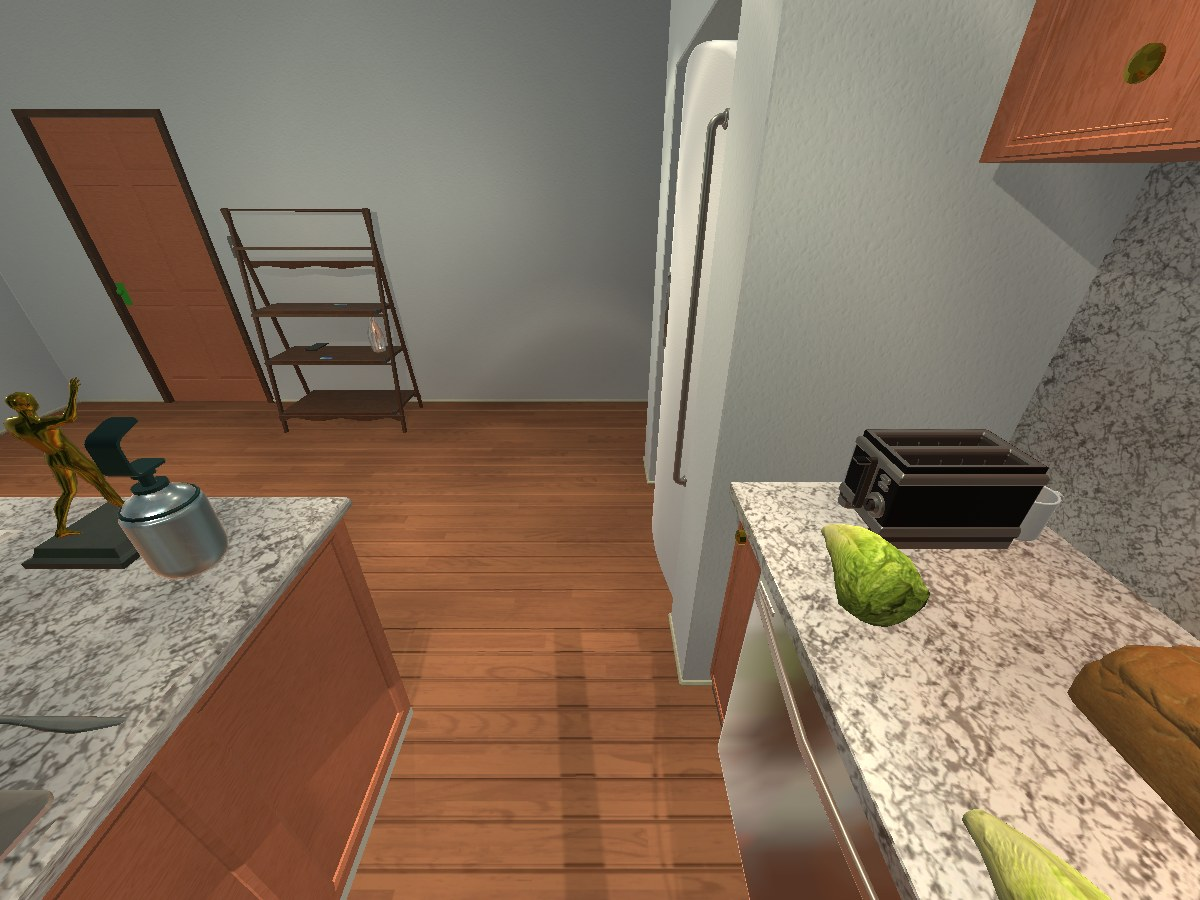
\includegraphics[width=8.815cm]{figures/cases/cool_view1.jpg}};
\draw[black!35, line width=0.4pt] (0.000,0.000) rectangle ++(8.815,-6.611);
\draw[dimF, line width=1.1pt] (7.628,-3.776) circle (0.238);
\draw[lead=dimF] (7.628,-3.776) -- (7.628,-3.276);
\fill[dimF] (7.628,-3.776) circle (0.06);
\node[lblkey=dimF] at (7.628,-3.276) {mug};
\draw[dimA, line width=1.1pt, rounded corners=1pt] (5.377,-3.541) rectangle (8.807,-6.611);
\draw[lead=dimA] (7.092,-5.076) -- (6.653,-4.614);
\fill[dimA] (7.092,-5.076) circle (0.06);
\node[lblkey=dimA] at (6.653,-4.614) {countertop: the mug is here};
\draw[dimE, line width=1.1pt, rounded corners=1pt] (4.789,-0.301) rectangle (5.414,-4.385);
\draw[lead=dimE] (5.102,-2.343) -- (5.102,-1.843);
\fill[dimE] (5.102,-2.343) circle (0.06);
\node[lblkey=dimE] at (5.102,-1.843) {fridge: cool it here};
\draw[liftpositive, line width=1.1pt, rounded corners=1pt] (7.316,-0.007) rectangle (8.807,-1.161);
\draw[lead=liftpositive] (8.062,-0.584) -- (7.068,-0.230);
\fill[liftpositive] (8.062,-0.584) circle (0.06);
\node[lblkey=liftpositive] at (7.068,-0.230) {cabinet: put it here};
\fill[black!55] (1.216,-5.079) circle (0.06);
\node[lbl=black!45] at (1.216,-5.079) {countertop};
\draw[lead=black!55] (6.931,-3.596) -- (6.664,-3.134);
\fill[black!55] (6.931,-3.596) circle (0.06);
\node[lbl=black!45] at (6.664,-3.134) {toaster};
\draw[lead=black!55] (5.399,-4.587) -- (5.399,-4.087);
\fill[black!55] (5.399,-4.587) circle (0.06);
\node[lbl=black!45] at (5.399,-4.087) {cabinet};
\node[anchor=north west, inner sep=0] at (9.065,0.000) {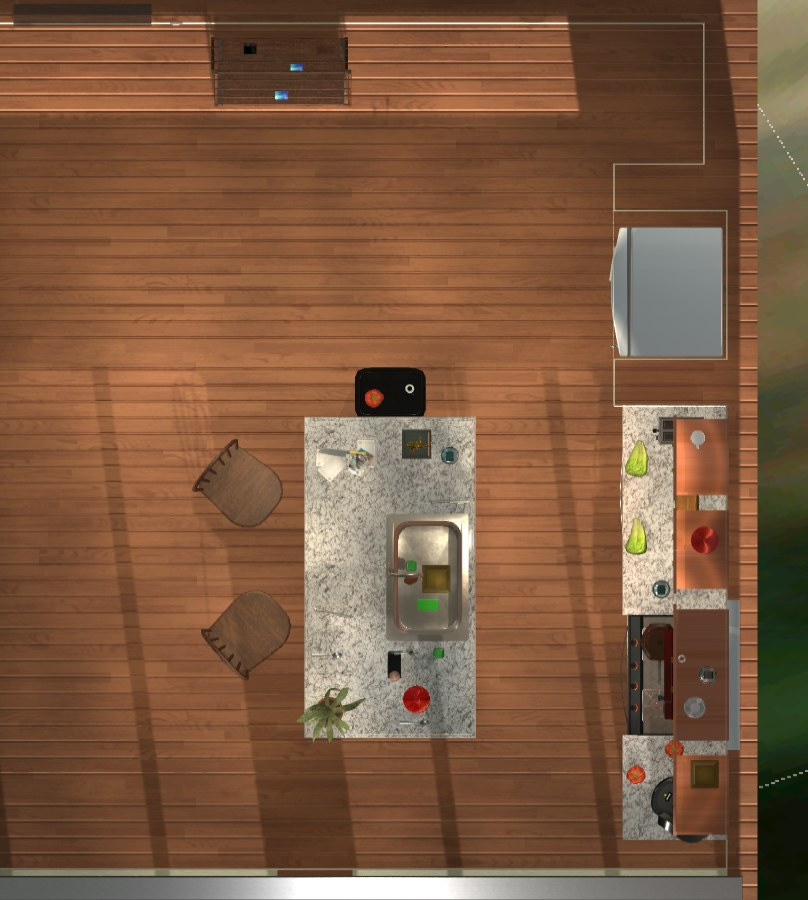
\includegraphics[width=5.935cm]{figures/cases/cool_map.jpg}};
\draw[black!35, line width=0.4pt] (9.065,0.000) rectangle ++(5.935,-6.611);
\fill[black, opacity=0.22] (13.252,-4.077) -- ++(45:1.1) arc (45:135:1.1) -- cycle;
\fill[black] (13.252,-4.077) circle (0.08);
\draw[white, line width=3.4pt, opacity=0.85] (14.008,-3.555) -- (14.035,-2.394);
\draw[path] (14.008,-3.555) -- (14.035,-2.394);
\draw[white, line width=3.4pt, opacity=0.85] (14.038,-2.344) -- (14.025,-3.430);
\draw[path] (14.038,-2.344) -- (14.025,-3.430);
\draw[lead=dimA] (14.003,-3.755) -- (12.803,-3.402);
\fill[dimA] (14.003,-3.755) circle (0.06);
\node[lblkey=dimA] at (12.803,-3.402) {countertop: the mug is here};
\draw[lead=dimE] (14.041,-2.144) -- (13.662,-1.682);
\fill[dimE] (14.041,-2.144) circle (0.06);
\node[lblkey=dimE] at (13.662,-1.682) {fridge: cool it here};
\draw[lead=liftpositive] (14.022,-3.680) -- (13.528,-2.941);
\fill[liftpositive] (14.022,-3.680) circle (0.06);
\node[lblkey=liftpositive] at (13.528,-2.941) {cabinet: put it here};
\draw[lead=black!55] (13.857,-3.809) -- (14.132,-4.271);
\fill[black!55] (13.857,-3.809) circle (0.06);
\node[lbl=black!45] at (14.132,-4.271) {cabinets};
\draw[lead=black!55] (13.912,-5.682) -- (13.912,-5.182);
\fill[black!55] (13.912,-5.682) circle (0.06);
\node[lbl=black!45] at (13.912,-5.182) {cabinets};
\draw[lead=black!55] (14.098,-5.925) -- (12.896,-5.734);
\fill[black!55] (14.098,-5.925) circle (0.06);
\node[lbl=black!45] at (12.896,-5.734) {coffeemachine};
\draw[lead=black!55] (11.611,-4.235) -- (10.913,-3.881);
\fill[black!55] (11.611,-4.235) circle (0.06);
\node[lbl=black!45] at (10.913,-3.881) {countertop};
\draw[lead=black!55] (14.003,-5.786) -- (13.305,-6.140);
\fill[black!55] (14.003,-5.786) circle (0.06);
\node[lbl=black!45] at (13.305,-6.140) {countertop};
\draw[lead=black!55] (13.679,-4.242) -- (12.779,-4.433);
\fill[black!55] (13.679,-4.242) circle (0.06);
\node[lbl=black!45] at (12.779,-4.433) {drawers};
\draw[lead=black!55] (11.933,-2.891) -- (11.933,-2.391);
\fill[black!55] (11.933,-2.891) circle (0.06);
\node[lbl=black!45] at (11.933,-2.391) {garbagecan};
\draw[lead=black!55] (14.125,-4.954) -- (14.125,-3.854);
\fill[black!55] (14.125,-4.954) circle (0.06);
\node[lbl=black!45] at (14.125,-3.854) {microwave};
\draw[lead=black!55] (11.115,-0.530) -- (10.215,-0.339);
\fill[black!55] (11.115,-0.530) circle (0.06);
\node[lbl=black!45] at (10.215,-0.339) {shelves};
\draw[lead=black!55] (12.207,-4.239) -- (11.207,-4.430);
\fill[black!55] (12.207,-4.239) circle (0.06);
\node[lbl=black!45] at (11.207,-4.430) {sinkbasin};
\draw[lead=black!55] (14.034,-4.960) -- (12.426,-4.960);
\fill[black!55] (14.034,-4.960) circle (0.06);
\node[lbl=black!45] at (12.426,-4.960) {stoveburners};
\draw[lead=black!55] (14.060,-3.164) -- (14.060,-2.364);
\fill[black!55] (14.060,-3.164) circle (0.06);
\node[lbl=black!45] at (14.060,-2.364) {toaster};
\node[imgcap] at (4.407,-6.651) {first-person view inside the room};
\node[imgcap] at (12.032,-6.651) {the room from above; cone: the left view; arrow: the expert's route};
\node[anchor=west, font=\sffamily\bfseries\footnotesize, text=black!70] at (0,-7.411) {Expert solution (6 steps):};
\node[chip, anchor=west] (s0) at (3.900,-7.411) {go to countertop};
\node[chip, anchor=west] (s1) at (6.872,-7.411) {take mug from countertop};
\draw[flow] (s0.east) -- (s1.west);
\node[chip, anchor=west] (s2) at (10.980,-7.411) {go to fridge};
\draw[flow] (s1.east) -- (s2.west);
\node[chip, anchor=west] (s3) at (3.900,-7.911) {cool mug with fridge};
\node[chip, anchor=west] (s4) at (7.440,-7.911) {go to cabinet};
\draw[flow] (s3.east) -- (s4.west);
\node[chip, anchor=west] (s5) at (9.986,-7.911) {move mug to cabinet};
\draw[flow] (s4.east) -- (s5.west);
\node[ptitle] at (0.000,-8.711) {(b) Effect of the memory on this family, 3 demonstration pairs};
\node[txt, text=black!65] at (0.000,-9.161) {family success: GPT $0.857\rightarrow0.746$, Qwen $0.857\rightarrow0.857$};
\draw[black!45] (7.400,-9.561) -- (7.400,-12.351);
\node[font=\sffamily\scriptsize, text=black!50] at (5.000,-12.521) {$-1$};
\node[font=\sffamily\scriptsize, text=black!50] at (7.400,-12.521) {$0$};
\node[font=\sffamily\scriptsize, text=black!50] at (9.800,-12.521) {$+1$};
\node[lab] at (4.850,-9.831) {task 5};
\fill[gptblue!55] (7.400,-9.681) rectangle ++(-1.200,-0.24);
\node[anchor=east, font=\sffamily\scriptsize, text=black!70] at (6.140,-9.801) {$-0.500$};
\fill[qwenmint!55] (7.400,-9.971) rectangle ++(-0.799,-0.24);
\node[anchor=east, font=\sffamily\scriptsize, text=black!70] at (6.541,-10.091) {$-0.333$};
\node[lab] at (4.850,-10.491) {task 16};
\fill[gptblue!55] (7.400,-10.341) rectangle ++(-0.799,-0.24);
\node[anchor=east, font=\sffamily\scriptsize, text=black!70] at (6.541,-10.461) {$-0.333$};
\fill[qwenmint!55] (7.400,-10.631) rectangle ++(0.000,-0.24);
\node[anchor=west, font=\sffamily\scriptsize, text=black!70] at (7.460,-10.751) {$0$};
\node[lab] at (4.850,-11.151) {task 19};
\fill[gptblue!55] (7.400,-11.001) rectangle ++(-0.799,-0.24);
\node[anchor=east, font=\sffamily\scriptsize, text=black!70] at (6.541,-11.121) {$-0.333$};
\fill[qwenmint!55] (7.400,-11.291) rectangle ++(0.000,-0.24);
\node[anchor=west, font=\sffamily\scriptsize, text=black!70] at (7.460,-11.411) {$0$};
\node[lab] at (4.850,-11.811) {task 39};
\fill[gptblue!55] (7.400,-11.661) rectangle ++(0.000,-0.24);
\node[anchor=west, font=\sffamily\scriptsize, text=black!70] at (7.460,-11.781) {$0$};
\fill[qwenmint!55] (7.400,-11.951) rectangle ++(0.799,-0.24);
\node[anchor=west, font=\sffamily\scriptsize, text=black!70] at (8.259,-12.071) {$+0.333$};
\fill[gptblue!55] (0.000,-9.911) rectangle ++(0.28,-0.18);
\node[txt] at (0.320,-10.001) {GPT-4o-mini};
\fill[qwenmint!55] (0.000,-10.311) rectangle ++(0.28,-0.18);
\node[txt] at (0.320,-10.401) {Qwen3-8B};
\end{scope}
\end{tikzpicture}
